\documentclass[]{book}
\usepackage{lmodern}
\usepackage{amssymb,amsmath}
\usepackage{ifxetex,ifluatex}
\usepackage{fixltx2e} % provides \textsubscript
\ifnum 0\ifxetex 1\fi\ifluatex 1\fi=0 % if pdftex
  \usepackage[T1]{fontenc}
  \usepackage[utf8]{inputenc}
\else % if luatex or xelatex
  \ifxetex
    \usepackage{mathspec}
  \else
    \usepackage{fontspec}
  \fi
  \defaultfontfeatures{Ligatures=TeX,Scale=MatchLowercase}
\fi
% use upquote if available, for straight quotes in verbatim environments
\IfFileExists{upquote.sty}{\usepackage{upquote}}{}
% use microtype if available
\IfFileExists{microtype.sty}{%
\usepackage{microtype}
\UseMicrotypeSet[protrusion]{basicmath} % disable protrusion for tt fonts
}{}
\usepackage[margin=1in]{geometry}
\usepackage{hyperref}
\hypersetup{unicode=true,
            pdftitle={Gridded GDP projections compatible with the five SSPs},
            pdfauthor={Global Carbon Project (Tsukuba International Office), NIES and ISM, Japan},
            pdfborder={0 0 0},
            breaklinks=true}
\urlstyle{same}  % don't use monospace font for urls
\usepackage{natbib}
\bibliographystyle{apalike}
\usepackage{longtable,booktabs}
\usepackage{graphicx,grffile}
\makeatletter
\def\maxwidth{\ifdim\Gin@nat@width>\linewidth\linewidth\else\Gin@nat@width\fi}
\def\maxheight{\ifdim\Gin@nat@height>\textheight\textheight\else\Gin@nat@height\fi}
\makeatother
% Scale images if necessary, so that they will not overflow the page
% margins by default, and it is still possible to overwrite the defaults
% using explicit options in \includegraphics[width, height, ...]{}
\setkeys{Gin}{width=\maxwidth,height=\maxheight,keepaspectratio}
\IfFileExists{parskip.sty}{%
\usepackage{parskip}
}{% else
\setlength{\parindent}{0pt}
\setlength{\parskip}{6pt plus 2pt minus 1pt}
}
\setlength{\emergencystretch}{3em}  % prevent overfull lines
\providecommand{\tightlist}{%
  \setlength{\itemsep}{0pt}\setlength{\parskip}{0pt}}
\setcounter{secnumdepth}{5}
% Redefines (sub)paragraphs to behave more like sections
\ifx\paragraph\undefined\else
\let\oldparagraph\paragraph
\renewcommand{\paragraph}[1]{\oldparagraph{#1}\mbox{}}
\fi
\ifx\subparagraph\undefined\else
\let\oldsubparagraph\subparagraph
\renewcommand{\subparagraph}[1]{\oldsubparagraph{#1}\mbox{}}
\fi

%%% Use protect on footnotes to avoid problems with footnotes in titles
\let\rmarkdownfootnote\footnote%
\def\footnote{\protect\rmarkdownfootnote}

%%% Change title format to be more compact
\usepackage{titling}

% Create subtitle command for use in maketitle
\newcommand{\subtitle}[1]{
  \posttitle{
    \begin{center}\large#1\end{center}
    }
}

\setlength{\droptitle}{-2em}

  \title{Gridded GDP projections compatible with the five SSPs}
    \pretitle{\vspace{\droptitle}\centering\huge}
  \posttitle{\par}
    \author{Global Carbon Project (Tsukuba International Office), NIES and ISM, Japan}
    \preauthor{\centering\large\emph}
  \postauthor{\par}
      \predate{\centering\large\emph}
  \postdate{\par}
    \date{February, 2020}

\usepackage{booktabs}
\usepackage{amsthm}
\makeatletter
\def\thm@space@setup{%
  \thm@preskip=8pt plus 2pt minus 4pt
  \thm@postskip=\thm@preskip
}
\makeatother

\begin{document}
\maketitle

{
\setcounter{tocdepth}{1}
\tableofcontents
}
\hypertarget{downscaling-gdp}{%
\chapter*{Downscaling GDP}\label{downscaling-gdp}}
\addcontentsline{toc}{chapter}{Downscaling GDP}

Estimated GDPs by 1/12-degree grids during 1850---2100 by 10 year intervals. In the estimation, national GDP data (past data until 2010; future projection under SSPs after 2020) is downscaled considering spatial and economic interactions among cities, urban growth patterns compatible with SSPs, and other auxiliary geographic data (land cover, road network, etc.). Methods which we used are detaily described in our forthcoming paper and data: \textbf{Murakami, Yoshida, and Yamagata (202X)}.

\begin{figure}
\centering
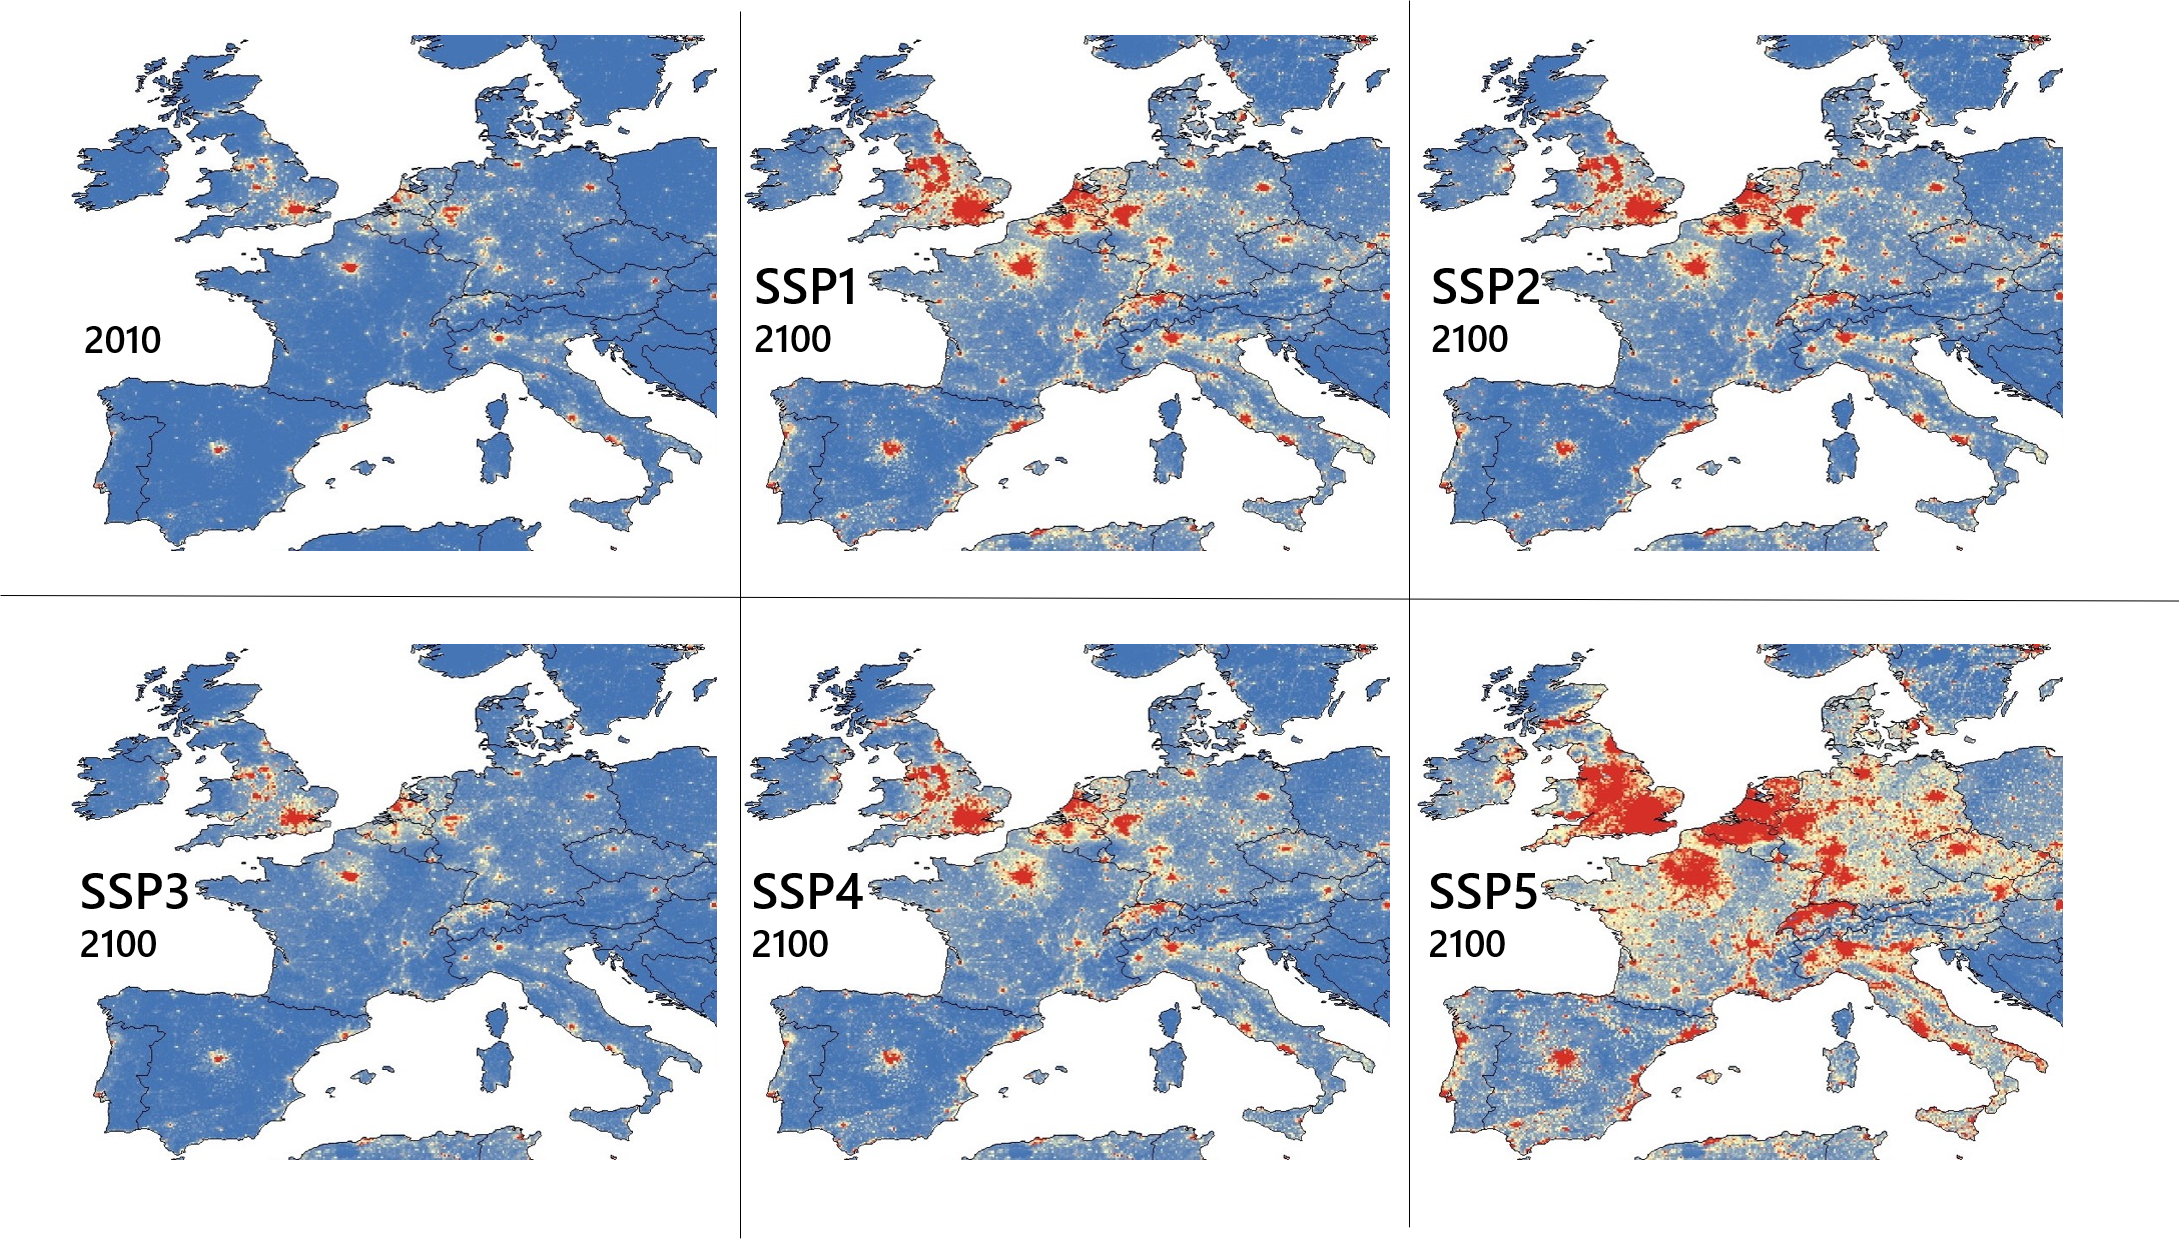
\includegraphics{Europe.png}
\caption{Figure: Europe in 2D}
\end{figure}

\begin{figure}
\centering
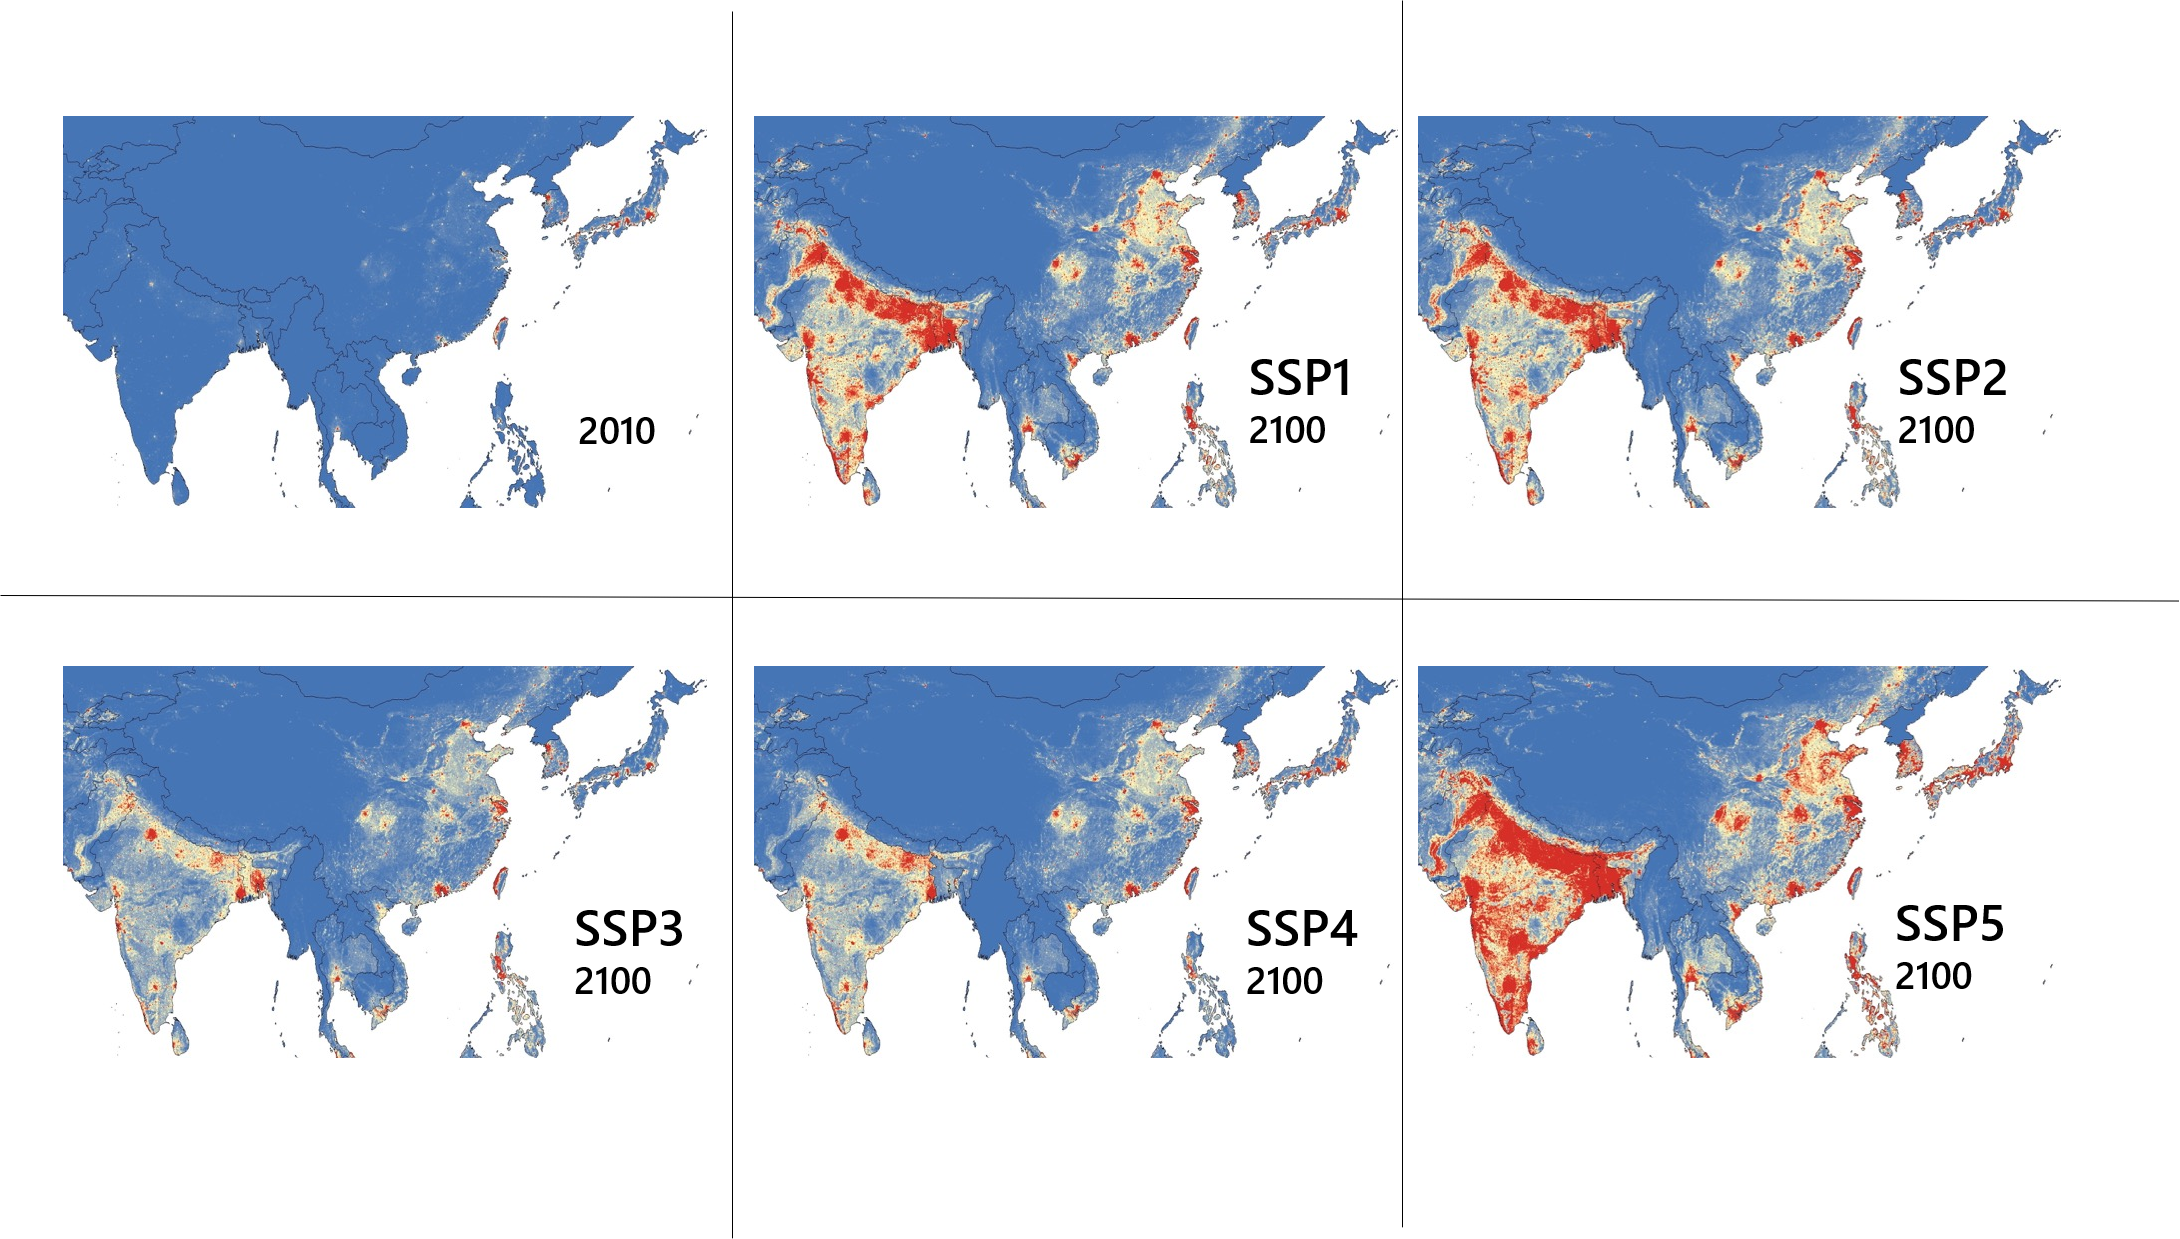
\includegraphics{Asia.png}
\caption{Figure: Asia in 2D}
\end{figure}

\begin{verbatim}
## PhantomJS not found. You can install it with webshot::install_phantomjs(). If it is installed, please make sure the phantomjs executable can be found via the PATH variable.
\end{verbatim}

\hypertarget{jDjXe8XbZ7}{}

Figure: Interactive 3D globe maping on downscaled GDP of SSP2-2100. You can pan and zoom the globe by mouse-over.

\begin{center}\rule{0.5\linewidth}{\linethickness}\end{center}

\hypertarget{data-download}{%
\section*{Data download}\label{data-download}}
\addcontentsline{toc}{section}{Data download}

The GDPs for SSP 1--5 between 2010 and 2100 by 10 years are estimated by 2160 x 4320 grids, each of which are 1/12-degree grids, covering the globe. The GDP estimates in each year in each SSP are recorded as a GeoTIff image with resolution of 2160 x 4320. GeoTiff is a Tiff image with spatial coordinates for each grid cell; the coordinates are given by longitude and latitude measured by World Geodetic System 1984 (WGS84).

\textbf{\emph{GeoTiff: please click here (PANGAEA)}} (please wait a moment. Now, we are uploading the data)

And also, you can download 3D globemap html files on the five SSPs (2010-2100) from the link below.

\textbf{\emph{3D globemaps: please click here}} (please wait a moment.)

\begin{center}\rule{0.5\linewidth}{\linethickness}\end{center}

\hypertarget{code-for-visualization}{%
\section*{Code for visualization}\label{code-for-visualization}}
\addcontentsline{toc}{section}{Code for visualization}

We used \href{https://www.r-project.org/}{\textbf{R}} for the 3D globe visualization.

\begin{verbatim}
library(colorRamps)
library(data.table)
library(dplyr)
library(htmlwidgets)
library(threejs)
library(tidyr)

setwd(****) # please set a directory including the file
dat <- data.table::fread(****) # please wait a moment!
# dat[1:3,]
#    longitude latitude gdp
# 1: -36.54172  83.5416   *
# 2: -36.45839  83.5416   *
# 3: -36.37506  83.5416   *

dat <- dat %>%
       dplyr::mutate(gdp=if_else(gdp>0,gdp,0)) %>%
       dplyr::filter(gdp>0) %>%
       dplyr::mutate(gdp.cut=as.numeric(cut(gdp,
        breaks=c(0,10^4,10^5,10^6,2.5*10^6,5.0*10^6,
                 10^7,2.5*10^7,5.0*10^7,10^8,10^9,max(gdp)), 
        include.lowest=TRUE))) %>%
       dplyr::mutate(pid=as.numeric(rownames(.))%%10) %>% # to avoid heavy calculation.
       dplyr::filter(pid==0)
3Dglobe <- threejs::globejs(lat=dat$latitude, long=dat$longitude,
        val=dat$gdp/10^7, # to adjust bar height 
        color=colorRamps::matlab.like(11)[dat$gdp.cut],
        pointsize=1.6,
        atmosphere=F)
3Dglobe        
\end{verbatim}

\begin{center}\rule{0.5\linewidth}{\linethickness}\end{center}

\hypertarget{references}{%
\section*{References}\label{references}}
\addcontentsline{toc}{section}{References}

\begin{itemize}
\tightlist
\item
  Daisuke Murakami, Takahiro Yoshida, Yoshiki Yamagata (202X) \textbf{Gridded GDP projections compatible with the five SSPs (Shared Socioeconomic Pathways)}. Submitted to \emph{a journal}.
\end{itemize}

\bibliography{book.bib,packages.bib}


\end{document}
